\chapter{Funciones de Lyapunov de Control}
\section{Función de Lyapunov de Control}

Este es quizá el método más general que se conoce para diseñar controladores para sistemas no lineales. En principio, si existe una forma de estabilizar un sistema no lineal, se puede \textit{siempre} usar este método. La idea en este capítulo es tratar de utilizar funciones de Lyapunov para hacer el diseño de un controlador.\\

\textbf{Motivación:}
\begin{itemize}
	\item Para $\dot{x} = f(x)$: Estabilidad asintótica $\Leftrightarrow$ Existe una \gls{fl}.
	\item Para $\dot{x} = f(x,u)$: Estabilizabilidad asintótica $\Leftrightarrow$ Existe una \gls{flc}.
\end{itemize}

Es importante entonces distinguir estos dos conceptos, que a priori parecerían lo mismo, pero cuando se tiene entrada no tiene mucho sentido hablar de \gls{fl}, sino de \gls{flc}. Por otro lado, el concepto de \gls{flc} no se aplica a sistemas que no tienen entrada de control.\\

Primero, consideremos el sistema \gls{si}, sin pérdida de generalidad para el caso de múltiples:
\begin{equation}
	\begin{aligned}
		\dot{x} & = f(x) + g(x)u                                         \\
		f(0)    & = 0, \quad x \in \mathbb{R}^n, \quad u \in \mathbb{R},
	\end{aligned}
\end{equation}
y suponga que existe una ley de control por retroalimentación de los estados:
\begin{equation*}
	u = \psi(x),
\end{equation*}
continua, tal que el origen del sistema en lazo cerrado
\begin{equation}
	\dot{x} = f(x) + g(x)\psi(x)
\end{equation}
es asintóticamente estable. Note que esta estabilización se puede llevar a cabo a través de múltiples controladores, y para cada uno de ellos se puede encontrar una \gls{fl} del lazo cerrado (que se considera como un sistema sin entrada).\\

Por el teorema converso de Lyapunov, sabemos que existe una función de Lyapunov $V(x)$ tal que
\begin{equation}
	\dfrac{\partial V(x)}{\partial x} [f(x) + g(x)\psi(x)] < 0, \quad \forall x \in D, x \neq 0
	\label{eq: converso_lyap1}
\end{equation}
Si $u = \psi(x)$ estabiliza globalmente al origen, entonces $D = \mathbb{R}^n$ y $V(x)$ es \gls{rna}.\\

De la desigualdad \eqref{eq: converso_lyap1} se concluye que
\begin{equation}
	\dfrac{\partial V(x)}{\partial x} g(x) = 0, \quad \text{para algún} \quad x \in D, x \neq 0 \Rightarrow \dfrac{\partial V(x)}{\partial x} f(x) < 0
	\label{eq: condicion_flc}
\end{equation}

En la expresión anterior, vea que nos interesa el signo de $\dfrac{\partial V(x)}{\partial x} f(x)$ en la variedad donde $\dfrac{\partial V(x)}{\partial x} g(x) = 0$.\\

Además, ya que $\psi(x)$ es continua, y $\psi(0) = 0, \forall \epsilon > 0, \exists \delta > 0$ tal que si $x \neq 0$ y $\|x\| < \delta$, existe $u$ con $\|u\| < \epsilon$ tal que

\begin{equation*}
	\dfrac{\partial V(x)}{\partial x} [f(x) + g(x)u] < 0
\end{equation*}

\rmk{Esta última es una condición adicional, y permite que el control sea continuo en el origen, y esta se conoce como la \gls{pcp}.}\\

\subsection{Interpretación Geométrica}

Por el \textbf{teorema converso de Lyapunov}, si logramos estabilizar el sistema mediante un control \( u = \psi(x) \), entonces existe una función de Lyapunov \( V(x) \) que satisface:

\begin{equation}
	\dot{V} = \underbrace{ \dfrac{\partial V}{\partial x} f(x) }_{\mathcal{V}(x)} +
	\underbrace{\dfrac{\partial V}{\partial x} g(x)}_{W(x)} \psi(x) < 0, \quad \forall x \in D, x \neq 0.
	\label{eq: lyapunov_interpretation}
\end{equation}

Analicemos el conjunto donde \( W(x) = 0 \). Este define una variedad de dimensión \( n-1 \) en \( \mathbb{R}^n \). Si tomamos un punto \( x^* \) en este conjunto, es decir, \( W(x^*) = 0 \), y \( V(x) \) es una \gls{fl} con el control \( \psi(x) \), entonces, ¿cómo debe ser \( \dot{V}(x^*) \)?  \textbf{Debe ser negativo}.\\

De la ecuación \eqref{eq: lyapunov_interpretation}, se concluye que el término \( \mathcal{V}(x^*) \) debe ser negativo. Es decir, en los puntos donde \( W(x) = 0 \), se cumple que \( \mathcal{V}(x) < 0 \). Además, el gradiente \( \frac{\partial V}{\partial x} \) es normal a una curva de nivel de \( V(x) \) y apunta hacia afuera de la misma. \\

Ahora, consideremos nuevamente el punto \( x^* \) donde \( W(x^*) = 0 \). En ese punto, \( V(x^*) \) tiene un valor asociado y existe una superficie de nivel que pasa por él. Por ejemplo, si \( V(x) \) es cuadrática, dicha superficie será una elipsoide. \\

En \( x^* \), el gradiente \( \frac{\partial V}{\partial x} \) apunta hacia afuera de la superficie de nivel. Si \( \mathcal{V}(x^*) \) es negativo, significa que \( f(x^*) \) apunta hacia adentro de la superficie de nivel, como se muestra en la Figura \ref{fig: lyapunov_interpretation}. En otras palabras, no importa cuál sea el control, en estos puntos el campo vectorial $f(x)$ impulsa a las trayectorias hacia dentro de la superficie de nivel, es decir, tiende a hacer que $V$ decrezca.

\rmkb{Note que no es necesario conocer el valor de $\psi(x)$, es decir, esta propiedad solo depende de $V(x)$ y de los campos vectoriales $f(x)$ y $g(x)$. Es decir, se puede checar esta condición sin necesidad de conocer el control.}\\

\begin{figure}[H]
	\centering
	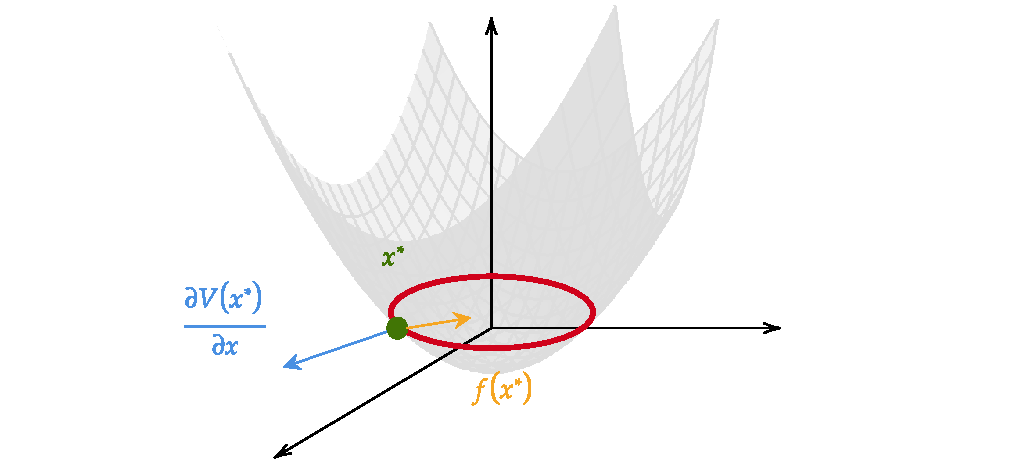
\includegraphics[width=0.75\textwidth]{img/flc_lyap_geom_interp.pdf}
	\caption{Interpretación geométrica de la función de Lyapunov de control.}
	\label{fig: lyapunov_interpretation}
\end{figure}


\rmk{
	Recuerde que aunque la interpretación geométrica es simple, no es fácil encontrar una \gls{flc}.\\
}

Un hecho sorprendente que se concluye de \ref{eq: condicion_flc} es que esto es una \textbf{condición necesaria y suficiente} para que $V(x)$ pueda ser una \gls{flc} para el sistema original, es decir, para que pueda existir una ley de control $\psi(x)$ que estabilice al origen. Si esta condición no se cumple, no puede existir tal ley de control, y esta condición se puede verificar sin necesidad de conocer a $\psi(x)$. De hecho, la existencia de una \gls{flc} es una caracterización de la estabilizabilidad para sistemas no lineales.\\
\rmkb{Entonces, cualquier \gls{fl} para el sistema en lazo cerrado con alguna ley de control que estabilice al origen es una \gls{flc} para el sistema original.}

\rmk{
	La caracterización es entonces extremadamente simple, pues uno no necesita conocer la ley de control para saber que \textbf{existe} una ley de control que estabiliza.
}

\defn{Función de Lyapunov de Control}{
	Una función $V(x)$, continuamente diferenciable y positiva definida, es una \gls{flc} para el sistema
	\begin{equation*}
		\dot{x} = f(x) + g(x)u
	\end{equation*}
	si
	\begin{itemize}
		\item \begin{equation}
			      \dfrac{\partial V(x)}{\partial x} g(x) = 0, \quad \text{para algún} \quad x \in D, x \neq 0 \Rightarrow \dfrac{\partial V(x)}{\partial x} f(x) < 0
			      \label{eq: condicion_flc2}
		      \end{equation}
		\item Satisface la \gls{pcp}.
	\end{itemize}
	Además, es una \gls{flc} global si es \gls{rna} y \eqref{eq: condicion_flc2} se satisface para $D = \mathbb{R}^n$.
}

\thmr{Teorema de Arstein}{arstein_thm}{
	Sea el sistema
	\begin{equation*}
		\dot{x} = f(x) + g(x)u,
	\end{equation*}
	con $f(0) = 0$. Entonces, el origen $x=0$ es \textbf{Globalmente Estabilizable Asintóticamente} por una ley de control de retroalimentación $u = \psi(x)$, continua en todas partes, excepto \textit{posiblemente} en el origen, si y solo si este posee una \gls{flc}. Si además se satisface la \gls{pcp}, entonces la ley de control puede ser continua en todas partes.
}

\section{Fórmula de Sontag}
\thmr{Fórmula de Sontag}{sontag_formula}{
	Sea $V(x)$ una \gls{flc} para el sistema
	\begin{equation*}
		\dot{x} = f(x) + g(x)u
	\end{equation*}
	entonces el origen es estabilizable por
	\begin{equation}
		u = \psi(x) = \begin{cases}
			\dfrac{-\frac{\partial V}{\partial x} f + \sqrt{\left(\frac{\partial V}{\partial x}f\right)^2 + \left(\frac{\partial V}{\partial x}g \right)^4}}{\left(\frac{\partial V}{\partial x}g\right)}, & \text{si } \frac{\partial V}{\partial x}g \neq 0 \\
			0,                                                                                                                                                                                             & \text{si } \frac{\partial V}{\partial x}g = 0.
		\end{cases}
		\label{eq: sontag_formula}
	\end{equation}

	Para el caso multivariable ($u \in \mathbb{R}^m$), se tiene que
	\begin{equation}
		u = \psi(x) = \begin{cases}
			\dfrac{L_f V(x) + \sqrt{[L_f V(x)]^2 + | L_g V(x) |^4}}{| L_g V(x) |^2}[L_g V(x)]^T, & \text{si } | L_g V(x) | \neq 0 \\
			0,                                                                                   & \text{si } | L_g V(x) | = 0.
		\end{cases}
		\label{eq: sontag_formula_multivariable}
	\end{equation}
}

\subsection{Una modificación de la fórmula de Sontag}
Elíjase una función $\gamma(x)$ tal que
\begin{itemize}
	\item $\gamma(x) \geq 0$ y $\gamma(0) = 0$.
	\item Si una solución acotada de la ecuación $\dot{x} = f(x)$ es tal que $\gamma(x(t)) \equiv 0$, entonces $x(t) \rightarrow 0$ cuando $t \rightarrow \infty$, por ejemplo, esto es cierto si $\gamma(x) > 0$ para $x \neq 0$ (detectable de estado cero).
\end{itemize}
\thmr{Fórmula de Sontag Modificada}{sontag_formula_mod}{
	Dada una \gls{flc} $V(x)$, considere la ley de control dada por
	\begin{equation}
		u = \psi(x) = \begin{cases}
			\dfrac{L_f V(x) + \sqrt{[L_f V(x)]^2 + \textcolor{red}{\gamma(x)}| L_g V(x) |\textcolor{red}{^2}}}{| L_g V(x) |^2}[L_g V(x)]^T, & \text{si } | L_g V(x) | \neq 0 \\
			0,                                                                                                                              & \text{si } | L_g V(x) | = 0.
		\end{cases}
		\label{eq: sontag_formula_mod}
	\end{equation}
}

\rmk{Nótese que:}
\begin{itemize}
	\item La elección de $\gamma(x) = |L_g V(x)|^2$ satisface los requisitos anteriores y se recupera la fórmula de Sontag.
	\item Hay muchas otras elecciones posibles de $\gamma(x)$: \textbf{Gran flexibilidad}.
\end{itemize}
\rmk{¿Cuáles son las propiedades de esta ley de control modificada?}
\begin{itemize}
	\item $\psi(x)$ hace que el \gls{pe} $x=0$ sea \gls{gae}.
	\item $\psi(x)$ es tan suave como $L_f V$, $L_g V$ y $\gamma(x)$, excepto (posiblemente) donde $\gamma(x) = L_f V (x) = 0$.
	\item Si $L_f V, L_g V$ y $\gamma(x)$ son localmente Lipschitz, entonces $\psi(x)$ también lo será, excepto (posiblemente) en el origen $x=0$.
	\item Si $V(x)$ tiene los mismos conjuntos de nivel que la solución de la ecuación de Hamilton-Jacobi-Bellman, asociada con la función de costo
	      \begin{equation*}
		      J = \int_0^\infty [\gamma(x(\tau)) + |u(\tau)|^2] d\tau
	      \end{equation*}
	      entonces $\psi(x)$ es óptima globalmente.
	\item Este hecho se puede usar para diseñar leyes de control localmente óptimas.
\end{itemize}

\rmkb{
	\textbf{Problema: ¿Cómo se puede encontrar una \gls{flc}?}

	Las propiedades de \gls{flc} y \gls{pcp} se preservan ante transformaciones de retroalimentación, es decir, retroalimentación y cambio de coordenadas (difeomórficas).\\

	Si se conoce algún control estabilizante y una \gls{fl} correspondiente $V$, entonces $V$ es una \gls{flc}.\\

	Principalmente, se verán dos formas de encontrar una \gls{flc}:
	\begin{itemize}
		\item Feedback Linearization
		\item Backstepping
	\end{itemize}
}



\subsection{FLC por Feedback Linearization}
Por este método es relativamente simple encontrar una \gls{flc}, ya que es muy simple estabilizar el sistema y encontrar una \gls{fl} para el sistema en lazo cerrado.\\

Considere el sistema
\begin{equation*}
	\dot{x} = f(x) + G(x)u, \quad z = T(x), \quad \dot{z} = (A-BK)z
\end{equation*}
Resolviendo la ecuación algrebraica de Lyapunov
\begin{equation*}
	(A-BK)^T P + P(A-BK) = -Q, \quad Q = Q^T > 0
\end{equation*}
Entonces
\begin{equation*}
	V(x) = z^T P z = T(x)^T P T(x)
\end{equation*}
es una \gls{flc} para el sistema original.\\

\rmkb{
	Una ley de control estabilizante alternativa para sistemas linealizables exactamente se puede obtener de la siguiente manera:
	\begin{itemize}
		\item Encuentre una \gls{flc} para el sistema \gls{lit} transformado (resolviendo la ecuación algebraica de Lyapunov).
		\item Use la fórmula de Sontag en vez de la ley de control linealizante.
	\end{itemize}
}

\ex{
	\begin{equation*}
		\dot{x} = ax - bx^3 + u, \quad a, b > 0
	\end{equation*}
	Linealización por retroalimentación:
	\begin{equation*}
		u = -(k+a)x + bx^3, \quad k > 0, \quad \Rightarrow \quad \dot{x} = -kx
	\end{equation*}
	Entonces, $V(x) = \dfrac{1}{2}x^2$ es una \gls{flc}.\\
	Luego,
	\begin{equation*}
		\dfrac{\partial V(x)}{\partial x} g(x) = x, \quad \dfrac{\partial V(x)}{\partial x} f(x) = x(ax - bx^3)
	\end{equation*}
	Usando la fórmula de Sontag:
	\begin{equation*}
		\begin{aligned}
			\psi(x) & = -\dfrac{x(ax - bx^3) + \sqrt{x^2(ax - bx^3)^2 + x^4}}{x} \\
			        & = -ax + bx^3 - x\sqrt{(a-bx^2)^2 + 1}
		\end{aligned}
	\end{equation*}
	Compare lo anterior con
	\begin{equation*}
		u = -ax + bx^3 -kx, \quad k > 0
	\end{equation*}
}

\lem{}{
	Sea $V(x)$ una \gls{flc} para el sistema
	\begin{equation*}
		\dot{x} = f(x) + g(x)u
	\end{equation*}
	y supóngase que
	\begin{equation*}
		\dfrac{\partial V(0)}{\partial x} = 0,
	\end{equation*}
	entonces la fórmula de Sontag tiene un margen de ganancia de $[\frac{1}{2},\infty]$, es decir, $u = k\psi(x)$ es estabilizante para toda $k \geq \frac{1}{2}$.
}








